\documentclass[12pt,twocolumn]{article}
\usepackage{tgtermes}
\usepackage[a4paper,left = 2cm,right = 1cm,top = 0cm,bottom = 1cm]{geometry}
\usepackage{amsmath}
\usepackage{graphicx}
\usepackage{amssymb}
\begin{document}
\large \title{ASSIGNMENT 1}
\author{Akhila (CS21BTECH11031)}
\maketitle
{\Large \textbf  {Que 10(a): }}
Use remainder theorem to factorize the following polynomial:\\
$f(x)=2x^3+3x^2-9x-10$.\\
\vspace{2mm}

{\Large \textbf  {Solution:}}
Let $f(x)=2x^3+3x^2-9x-10$ 

Put $x=-1$ we get,
\begin{align*}
f(-1) & =2(-1)^3+3(-1)^2-9(-1)-10\\
      & =-2+3+9-10\\ 
      & =0
\end{align*}
So, $(x+1)$ is a factor of $f(x)$.

Dividing $f(x)$ with $(x+1)$\\ 
 we get,
\begin{equation*}
    f(x)=(x+1)(2x^2+x-10)
\end{equation*}
The term $(2x^2+x-10)$ can be factorized as
\begin{equation*}
    (2x^2+5x-4x-10)=(x-2)(2x+5)
\end{equation*}
\vspace{5mm}
$\therefore f(x)=(x+1)(x-2)(2x+5)$\\
Hence,  $(x+1)$,$(x-2)$ and $(2x+5)$  are the factors of the given polynomial\\
$2x^3+3x^2-9x-10$.
\begin{figure}
\centering
    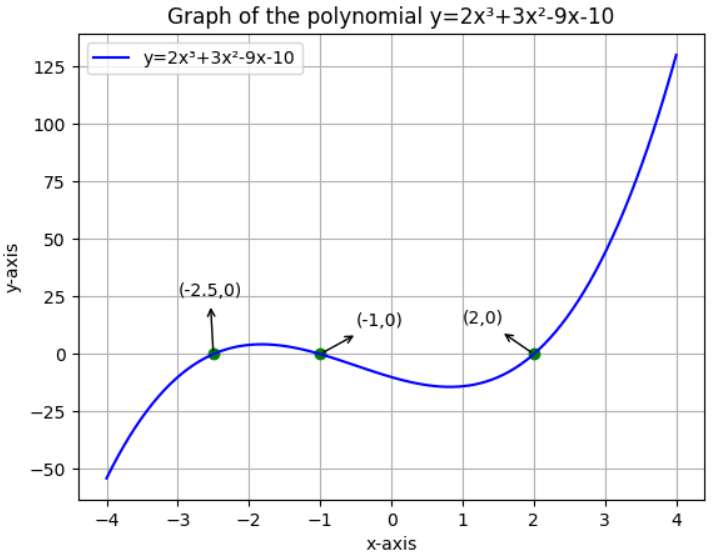
\includegraphics[scale=0.5]{plot1.png}
\end{figure}
\end{document}
